El proyecto no se ha desarrollado siguiendo un calendario estricto,
dado que era imposible cuantificar el tiempo que tomaría el adquirir
las bases teóricas necesarias para poder afrontarlo con garantías. Su
desarrollo se ha compaginado con los estudios del último curso de
Ingeniería Técnica en Informática de Sistemas y las labores como
becario en la Oficina de Software Libre y Conocimiento Abierto de la
Universidad de Cádiz~\cite{osluca}.

\section{Iteraciones}
Para la realización del proyecto se ha utilizado un modelo de desarrollo
iterativo incremental. En la redacción del presente documento se presentarán la
fase de investigación preliminar y las etapas de análisis, diseño,
implementación y pruebas del proyecto en su estado final. A continuación se
detallan cada una de las iteraciones por las que ha ido pasando el proyecto.

\subsection{Primera iteración: conocimientos preliminares}
Antes de poder comenzar con el análisis y diseño del propio proyecto,
era esencial adquirir una serie de conocimientos para poder afrontar
su desarrollo con todas las garantías. Durante esta iteración, se
llevaron a cabo labores de documentación y aprendizaje autodidacta con
las que se asentaron los conocimientos necesarios.

Además, durante este periodo también se barajaron las diferentes
posibilidades de implementación del sistema, así como las posibles
herramientas y bibliotecas de terceros que pudieran ser de ayuda.

\subsection{Segunda iteración: analizador básico}
Una vez adquiridos los conocimientos teóricos necesarios, y decididas
las técnicas y herramientas para llevar aquellos a la práctica, fue
obvia la necesidad de empezar por diseñar un analizador de notas
básico, que sería el corazón del programa. Del éxito del desarrollo
temprano del módulo que se encargaría del análisis de sonidos
dependería la viabilidad completa del proyecto.

\subsection{Tercera iteración: interfaz gráfica de usuario}
Con el módulo de análisis desarrollado, \textit{sólo} restaba
desarrollar el resto de la aplicación alrededor del mismo. En esta
tercera iteración se propusieron numerosos diseños para la interfaz
gráfica de usuario y, una vez decantados por uno de ellos, comenzó el
desarrollo de los elementos de la interfaz, haciendo énfasis en
conseguir un aspecto dinámico y jovial.

\subsection{Cuarta iteración: motor de lecciones}
Uno de los subproductos de la aplicación es el motor de lecciones, que
presenta una serie de unidades didácticas en formato multimedia,
compuestas de imágenes y textos, con conceptos sobre música. En esta
iteración se hizo un análisis de las posibilidades de este motor,
concluyendo con el diseño y desarrollo de un mecanismo muy sencillo de
ampliar y utilizar.

\subsection{Quinta iteración: motor de canciones}
La parte de mayor interactividad de la aplicación es el motor de
canciones, en el que el usuario tiene la posibilidad de tocar una
canción que aparece en pantalla, usando la flauta, mientras la
aplicación valora en tiempo real su interpretación. Durante la quinta
iteración se elaboró este sistema, encargado de listar y cargar las
diferentes canciones, y puntuar al usuario según cómo lo haga.

\section{Diagrama de Gantt}
Se ha diseñado un diagrama de Gantt para reflejar la distribución de las tareas
a lo largo del tiempo (figura~\ref{fig:gantt} en la página~\pageref{fig:gantt}).

\begin{figure}
  \centering
  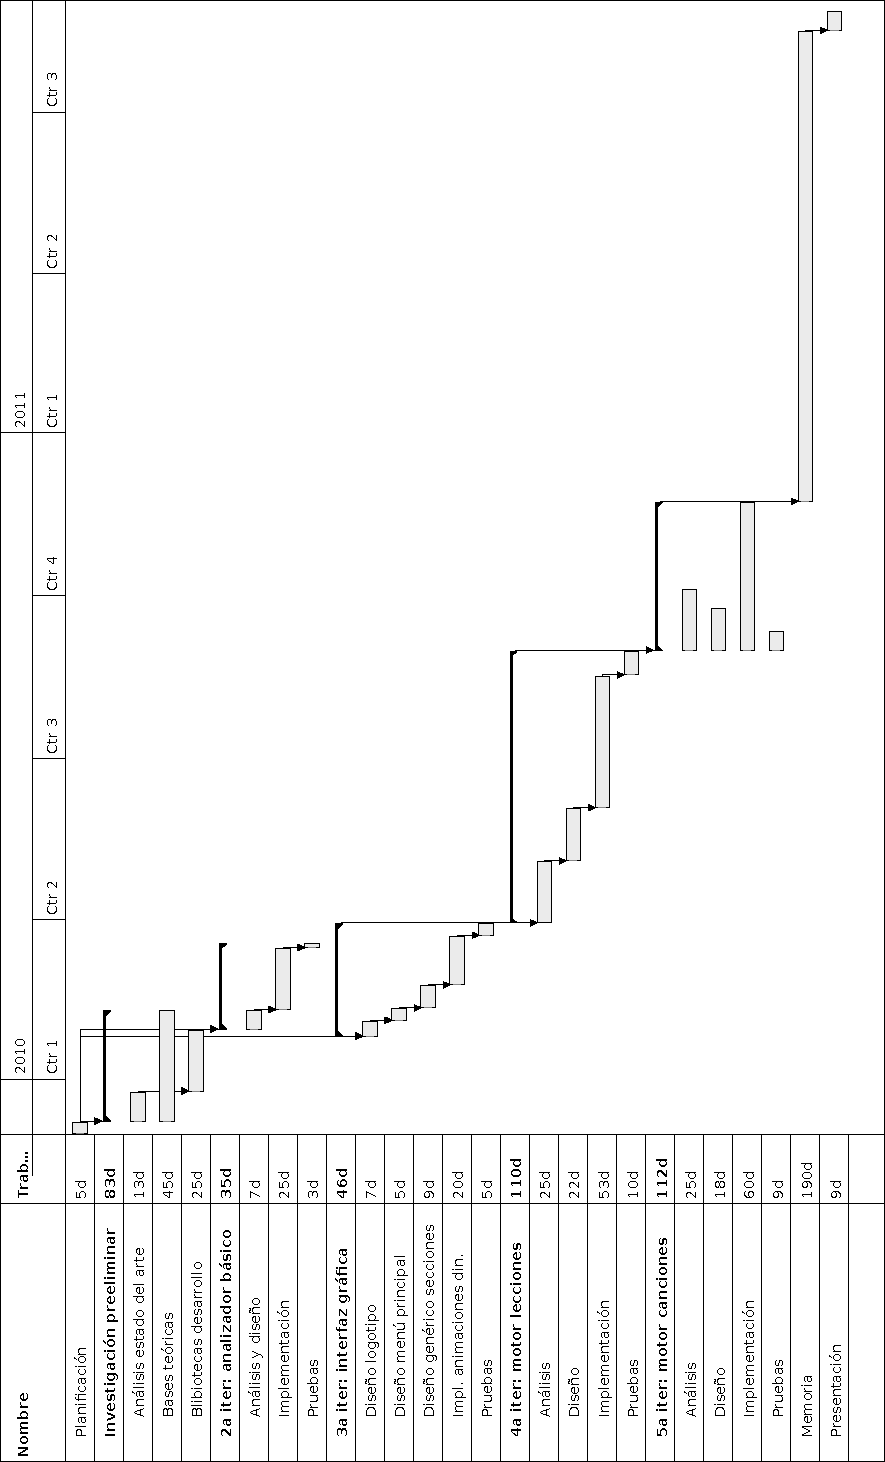
\includegraphics[width=0.95\textwidth]{2_calendario/imagen_diagrama_gantt}
  \caption{Diagrama Gantt de iteraciones}
  \label{fig:gantt}
\end{figure}

%%% Local Variables: 
%%% mode: latex
%%% TeX-master: "../memoria"
%%% End: 
